\chapter{Аналитический раздел}

\section{Анализ задачи}

Задача декомпозиции сложных вопросов может быть определена как преобразование исходного вопроса в набор более простых, где каждый простой вопрос направлен на получение части информации, необходимой для полного ответа \cite{perez2020unsupervised}. При этом возникают следующие ключевые проблемы:

\begin{enumerate}
	\item определение границ подвопросов: необходимо корректно выделить независимые смысловые части исходного вопроса;
	\item сохранение контекста: простые вопросы должны сохранять связь с контекстом исходного вопроса;
	\item обеспечение полноты: набор простых вопросов должен покрывать всю информационную потребность исходного вопроса;
	\item устранение избыточности: необходимо избегать повторяющихся или пересекающихся подвопросов \cite{barhaim2020quantitative}.
\end{enumerate}

Особую сложность представляют вопросы, содержащие неявные логические связи, требующие понимания контекста и предметной области. Например, вопрос \enquote{Как повлияла индустриальная революция на развитие городов в Европе?} требует учета множества аспектов: экономических, социальных, технологических и демографических изменений.

\section{Анализ существующих решений}

\subsection{Экспертная оценка}

В области декомпозиции сложных вопросов базовым подходом является привлечение экспертов предметной области. Эксперты, опираясь на свои знания и опыт, способны эффективно разбивать сложные вопросы на простые составляющие, учитывая специфику области и контекст. Такой подход обеспечивает высокое качество декомпозиции и позволяет выявлять неочевидные связи между компонентами вопроса, однако имеет ограничения по масштабируемости и требует значительных временных и человеческих ресурсов. \cite{wang2022human}

\subsection{Алгоритмические методы}

\textbf{EDG-Based Question Decomposition} представляет собой комплексный подход к разбиению сложных вопросов, основанный на построении графа описания сущностей (Entity Description Graph). Алгоритм создаёт направленный ациклический граф, где узлы представляют вопросы и сущности, а рёбра отражают логические связи между ними. Особенность метода заключается в использовании итеративного процесса разбиения с применением специализированных правил: W-Rule для обработки вопросительных конструкций, C-Rule для координационных союзов, A-Rule и N-Rule для работы с атрибутивными и именными группами. Эффективность алгоритма подтверждена на задачах построения запросов к базам знаний, однако его производительность существенно зависит от качества начального синтаксического анализа. \cite{hu2021edg}

\textbf{Question Decomposition with Dependency Graphs} реализует подход на основе модели QDMR (Question Decomposition Meaning Representation), где сложный вопрос преобразуется в серию простых вычислительных шагов. Алгоритм применяет конвертацию аннотаций в логические формы и далее в dependency-графы, что позволяет явно моделировать связи между частями вопроса. Метод показывает 16-кратное ускорение по сравнению с другими моделями, однако требует качественной предварительной разметки данных для обучения. \cite{hasson2021question}

\textbf{SPARQA: Skeleton-based Semantic Parsing} предлагает подход к декомпозиции вопросов через построение \enquote{скелета} -- формализации на основе dependency-грамматики. Алгоритм итеративно разбивает вопрос на текстовые span'ы, определяя их взаимосвязи и формируя направленное дерево. Особенность метода заключается в фокусировке на высокоуровневой семантической организации вопроса, что позволяет избежать ошибок dependency-парсинга на длинных сложных конструкциях. Однако метод требует значительных вычислительных ресурсов для построения и анализа скелетной структуры. \cite{sun2020sparqa}

\textbf{Hierarchical Semantic Parsing (HSP)} реализует трёхэтапный подход к декомпозиции вопросов. На первом этапе специальная нейронная модель разбивает исходный вопрос на последовательность подвопросов, затем извлекается ключевая семантическая информация, и наконец происходит интеграция данных для построения логической формы. Метод отличается способностью генерировать полные, естественные подвопросы вместо простого поиска точек разделения, однако требует тщательной настройки параметров для достижения оптимальной производительности. \cite{zhang2019complex}

\subsection{Методы на основе больших языковых моделей}

Большие языковые модели (Large Language Models, LLM) представляют собой особый класс решений для декомпозиции сложных вопросов, не требующий предварительной разработки правил или алгоритмов. В отличие от традиционных подходов, языковые модели способны выполнять декомпозицию, основываясь только на текстовой инструкции (промпте) и собственном обучении на больших массивах текстовых данных. \cite{venktesh2023context} Данный подход значительно упрощает процесс внедрения и масштабирования решений для задач декомпозиции вопросов на практике.

\textbf{DeepSeek} (DeepSeek-V3-Chat) использует архитектуру смеси экспертов, что обеспечивает эффективное распределение вычислительных ресурсов при обработке запросов. Модель демонстрирует высокие результаты в задачах рассуждения и решения проблем, особенно в технических областях, где требуется понимание контекста и многоступенчатый анализ. \cite{deepseek}

\textbf{ChatGPT-4} (chatgpt-4o-latest) представляет собой мультимодальную модель от OpenAI, способную эффективно обрабатывать текст, изображения и аудио данные. Благодаря улучшенной архитектуре и оптимизированным механизмам обработки информации, модель показывает высокую производительность при сниженной стоимости использования по сравнению с предыдущими версиями, что делает её подходящей для широкого спектра приложений. \cite{gpt4}

\textbf{O1} (o1-mini) от OpenAI представляет собой компактную модель, оптимизированную для быстрого отклика и низких вычислительных затрат. Модель использует технологии квантования и дистилляции для достижения баланса между производительностью и качеством, что делает её эффективной для встраиваемых систем и мобильных приложений, где критична скорость работы и ограничены вычислительные ресурсы. \cite{o1}

\textbf{Yi-Lightning} (yi-lightning) использует архитектуру смеси экспертов с оптимизированной системой маршрутизации вычислений. Модель показывает высокие результаты в обработке китайского языка, математических вычислениях и задачах программирования, при этом обеспечивая эффективное использование вычислительных ресурсов. \cite{yi}

\textbf{Claude-3} (claude-3-opus-20240229) от Anthropic реализует комплексный подход к обработке текста и изображений. Модель демонстрирует высокие результаты в тестах MMLU и GPQA, что подтверждает её способность к качественному анализу и обработке сложных запросов в различных предметных областях. \cite{claude}

\textbf{T-Tech} (T-Tech-T-pro-it-1.0) ориентирована на промышленные приложения и обработку технической документации. Модель обучена на корпусе русского и английского языков, что позволяет ей эффективно работать с технической документацией и специализированными текстами в обоих языках. \cite{ttech}

\textbf{GigaChat} (SberDevices-GigaChatMax) представляет собой российскую разработку с расширенными возможностями обработки естественного языка. Модель эффективно справляется с задачами коммуникации на русском языке, генерацией программного кода и аналитической обработкой данных, что делает её востребованной в различных бизнес-приложениях. \cite{gigachat}

\textbf{Gemini} (gemini-1.5-pro-002) от Google обеспечивает комплексную обработку текста, кода и мультимодальных данных. Модель отличается улучшенной производительностью в тестах MMLU и MATH, а оптимизированная система обработки данных позволяет снизить затраты на использование при сохранении высокого качества результатов. \cite{gemini}

\textbf{Qwen} (Qwen2.5-72B-Instruct) от Alibaba поддерживает работу с 29 языками и обеспечивает высокое качество обработки естественного языка. Модель показывает стабильные результаты в задачах программирования и математических вычислениях, что делает её универсальным инструментом для различных прикладных задач. \cite{qwen}

\textbf{Phi} (Phi-4) от Microsoft представляет собой компактную модель с 14 миллиардами параметров. Благодаря специализированной подготовке на качественных наборах данных, модель демонстрирует высокую эффективность в решении математических задач и обработке научных текстов. \cite{phi}

\textbf{LLaMA 3} (llama-3.1-70b-instruct) от Meta обеспечивает высокую производительность в различных задачах обработки естественного языка. Модель успешно проходит тесты HumanEval и MMLU, что подтверждает её способность к анализу и генерации текста в различных предметных областях. \cite{llama}

\textbf{Mistral} (mistral-large-2407) реализует поддержку множества языков программирования и естественных языков. Модель обладает развитыми механизмами рассуждения и доступна через API на различных платформах, что упрощает её интеграцию в существующие системы. \cite{mistral}

\textbf{Command-R+} (command-r-plus) от Cohere разработана для решения корпоративных задач и поддерживает работу с десятью языками. Модель обеспечивает высокую пропускную способность и низкую задержку, что делает её эффективным инструментом для промышленного применения. \cite{cohere}

\textbf{Gemma-2} (gemma-2-9b-it) от Google представляет собой открытую модель, оптимизированную для практического применения. Модель показывает высокие результаты в тестах MMLU и адаптирована для работы как в облачной среде, так и на мобильных устройствах. \cite{gemma}

\textbf{Watari} (Watari-7b-v1) специализируется на обработке японского и английского языков с особым вниманием к языковым нюансам. Модель эффективно обрабатывает различные уровни вежливости в японском языке и поддерживает точный перевод между языками. \cite{watari}

\textbf{YandexGPT} (yandexgpt-4-pro) фокусируется на обработке русского языка и применяется в различных бизнес-задачах. Модель успешно используется для создания контента и разработки чат-ботов, демонстрируя высокую эффективность в задачах на русском языке. \cite{yandexgpt}

\textbf{GPT-3.5 Turbo} (gpt-3.5-turbo-0125) обеспечивает эффективную обработку текста при оптимальном соотношении цены и качества. Модель демонстрирует высокие результаты в тестах HellaSwag и MMLU, что подтверждает её способность к качественному анализу текста в различных контекстах. \cite{gpt35}

\textbf{GLM-4} (glm-4-9b-chat) поддерживает работу с 26 языками и обладает расширенным контекстным окном. Модель включает функционал веб-поиска и выполнения программного кода, что расширяет её возможности в решении практических задач. \cite{chatglm}

\textbf{C4AI Command-R} (c4ai-command-r-v01) оптимизирована для задач рассуждения и обработки текстов. Модель поддерживает работу с большими объемами контекста и включает механизмы проверки генерируемого содержания, что повышает надежность её использования. \cite{c4ai}

\textbf{Suzume} (suzume-llama-3-8b-multilingual) основана на архитектуре LLaMA-3 и адаптирована для многоязычного применения. Модель обучена на большом корпусе диалогов на разных языках, что обеспечивает высокое качество обработки естественного языка в многоязычных приложениях. \cite{suzume}

\textbf{Hermes-2} (hermes-2-theta-llama-3-8b) от Nous Research фокусируется на качественной обработке длительных диалогов. Модель эффективно сохраняет контекст беседы и поддерживает расширенные возможности взаимодействия с пользователем через программные интерфейсы. \cite{hermes}

\textbf{Saiga} (saiga\_llama3\_8b\_v6) разработана для работы с научной литературой в области точных наук. Модель обеспечивает точную обработку математических формул и поддерживает форматирование в LaTeX, что делает её полезным инструментом для научной работы. \cite{saiga}

\textbf{Aya-23-8b} (aya-23-8b) реализует поддержку 23 языков через систему специализированных адаптеров. Модель обеспечивает высокое качество обработки текста для каждого поддерживаемого языка, приближаясь по эффективности к специализированным одноязычным решениям. \cite{aya}

\textbf{Paralex} (paralex-llama-3-8b-sft) ориентирована на обработку юридической и финансовой документации. Модель обеспечивает высокую точность анализа документов и значительно ускоряет процессы их обработки по сравнению с универсальными решениями. \cite{paralex}

\textbf{Storm} (storm-7b) оптимизирована для работы в режиме реального времени на стандартном оборудовании. Модель сохраняет высокий уровень производительности при сниженных требованиях к вычислительным ресурсам, что делает её подходящей для широкого спектра применений. \cite{storm}

\textbf{Neural-Chat} (neural-chat-7b-v3-3) от Intel использует оптимизированные методы вычислений для повышения производительности. Модель поддерживает специализированные инструкции процессоров Intel и обеспечивает эффективную обработку данных на серверном оборудовании. \cite{neural}

\textbf{Vikhr} (vikhr-nemo-12b-instruct-r-21-09-24) представляет собой открытую модель для работы с русским языком. Модель использует специально адаптированную систему токенизации и постоянно совершенствуется через процесс непрерывного обучения. \cite{vikhr}

\textbf{RuadaptQwen} (RuadaptQwen-32B-Pro\_v1) представляет собой адаптированную для русского языка версию модели Qwen2.5-32B с усовершенствованным токенизатором. Модель демонстрирует значительное повышение скорости генерации русскоязычных текстов при сохранении высокого качества ответов и эффективно решает широкий спектр задач обработки естественного языка. \cite{ruadapt}

\textbf{Zero-Mistral} (ru-Zero-Mistral-Small-24B) основана на Mistral-Small-24B-Instruct-2501 с оптимизацией для русского и английского языков. Модель демонстрирует высокую производительность в задачах диалоговых систем и обеспечивает эффективную обработку запросов с сохранением контекста, что делает её подходящей для создания отзывчивых ассистентов. \cite{zeromistral}

\textbf{Cotype-Nano} (MTSAIR-Cotype-Nano) представляет собой легковесную модель, оптимизированную для работы в условиях ограниченных вычислительных ресурсов. Модель разработана с использованием двухэтапного обучения, где MLP-слои тренировались на математических задачах и программном коде, что обеспечивает эффективную обработку запросов на русском и английском языках при сохранении быстродействия. \cite{cotype}

\section{Сравнение больших языковых моделей}

Для объективной оценки возможностей языковых моделей была использована платформа LLM Arena -- открытая краудсорсинговая система оценки больших языковых моделей на русском языке. Платформа использует модель Брэдли-Терри для ранжирования моделей на основе парных сравнений, выполненных людьми, и представляет результаты по шкале Эло. Модель Брэдли-Терри позволяет трансформировать субъективные оценки экспертов в количественные показатели, где вероятность предпочтения одной модели над другой зависит от разницы их рейтингов.

В таблице \ref{tab:llm-comparison} представлены результаты тестирования лучших представителей каждого семейства моделей в категории Arena-Hard-Auto. Для каждой архитектуры или линейки моделей была отобрана версия с наивысшим показателем эффективности, что позволяет провести объективное сравнение различных подходов к построению языковых моделей. Представленные метрики включают: Score -- общий балл модели по шкале Эло, отражающий её относительную силу в сравнении с другими моделями; CI (Confidence Interval) -- доверительный интервал, указывающий на статистическую погрешность оценки; Avg Tokens -- среднее количество токенов в ответе, характеризующее детальность генерируемых текстов; SD (Standard Deviation) -- стандартное отклонение количества токенов, отражающее стабильность объёма ответов; LC (Language Competency) -- оценка языковой компетенции, представляющая собой нормализованный показатель способности модели работать с естественным языком. Высокие значения Score и LC обычно коррелируют с лучшим пользовательским восприятием качества ответов. \cite{llmarena}

\begin{table}[H]
	\caption{Рейтинг языковых моделей по результатам тестирования в LLM Arena}
	\label{tab:llm-comparison}
	\begin{tabular}{|l|c|c|c|c|c|}
		\hline
		\textbf{Модель} & \textbf{Score} & \textbf{CI} & \textbf{Avg Tokens} & \textbf{SD} & \textbf{LC} \\
		\hline
		DeepSeek-V3-Chat & 96.30 & +0.8/-0.7 & 665.97 & 504.83 & 56.62 \\
		chatgpt-4o-latest & 94.74 & +0.8/-1.0 & 693.15 & 634.20 & 56.40 \\
		o1-mini & 93.46 & +0.7/-0.8 & 791.18 & 647.74 & 56.22 \\
		yi-lightning & 93.46 & +0.9/-1.0 & 636.68 & 469.74 & 56.22 \\
		RuadaptQwen-32B-Pro\_v1 & 92.18 & +1.2/-1.2 & 563.43 & 387.83 & 56.04 \\
		claude-3-opus-20240229 & 91.31 & +1.0/-1.1 & 468.69 & 254.10 & 55.92 \\
		T-Tech-T-pro-it-1.0 & 90.87 & +0.8/-1.1 & 502.00 & 380.68 & 55.85 \\
		SberDevices-GigaChatMax & 89.96 & +1.2/-1.4 & 523.95 & 421.87 & 55.73 \\
		gemini-1.5-pro-002 & 89.07 & +1.3/-0.9 & 639.51 & 493.30 & 55.60 \\
		Qwen2.5-72B-Instruct & 88.25 & +0.8/-1.5 & 557.41 & 437.32 & 55.48 \\
		ru-Zero-Mistral-Small-24B & 87.43 & +1.4/-1.2 & 565.19 & 339.27 & 55.37 \\
		vikhr-nemo-12b-instruct-r & 87.31 & +1.1/-1.4 & 627.00 & 416.72 & 55.35 \\
		Phi-4 & 86.59 & +1.1/-1.3 & 641.70 & 439.80 & 55.25 \\
		llama-3.1-70b-instruct & 83.26 & +1.4/-1.1 & 537.53 & 428.60 & 54.77 \\
		mistral-large-2407 & 80.40 & +2.1/-1.5 & 422.42 & 320.72 & 54.36 \\
		command-r-plus & 77.17 & +1.5/-1.5 & 560.83 & 424.07 & 53.90 \\
		gemma-2-9b-it & 76.50 & +1.3/-1.3 & 459.15 & 312.59 & 53.81 \\
		Watari-7b-v1 & 69.49 & +1.7/-1.7 & 616.80 & 449.25 & 52.80 \\
		yandexgpt-4-pro & 59.24 & +2.1/-1.9 & 383.80 & 306.97 & 51.33 \\
		MTSAIR-Cotype-Nano & 50.51 & +1.9 / -1.4 & 567.34 & 435.47 & 50.07 \\
		gpt-3.5-turbo-0125 & 50.00 & +0.0/-0.0 & 220.83 & 170.30 & 50.00 \\
		glm-4-9b-chat & 49.75 & +2.0/-2.0 & 568.81 & 448.76 & 49.96 \\
		c4ai-command-r-v01 & 48.95 & +3.0/-2.1 & 529.34 & 368.98 & 49.85 \\
		suzume-llama-3-8b & 45.71 & +2.3/-2.6 & 641.18 & 858.96 & 49.38 \\
		hermes-2-theta-llama-3-8b & 44.08 & +2.4/-2.3 & 485.99 & 390.85 & 49.15 \\
		saiga\_llama3\_8b\_v6 & 39.17 & +2.1/-1.6 & 471.51 & 463.62 & 48.44 \\
		aya-23-8b & 36.26 & +1.9/-2.2 & 554.34 & 433.51 & 48.02 \\
		paralex-llama-3-8b-sft & 37.36 & +2.5/-2.2 & 688.57 & 632.87 & 48.18 \\
		storm-7b & 20.62 & +1.7/-1.4 & 419.32 & 190.85 & 45.78 \\
		neural-chat-7b-v3-3 & 19.04 & +1.5/-1.5 & 927.21 & 1211.62 & 45.56 \\
		\hline
	\end{tabular}
\end{table}

\section{Модель разрабатываемого процесса}

Для наглядного представления процесса разбиения сложных вопросов на простые была создана IDEF0-диаграмма (рисунок \ref{fig:idef0}). На ней показано, как сложный вопрос преобразуется в набор простых вопросов.

После анализа всех рассмотренных методов, для решения задачи лучше всего подходят большие языковые модели. Это объясняется несколькими причинами:
\begin{itemize}
	\item отсутствие необходимости в разработке сложных правил и алгоритмов;
	\item высокая адаптивность к различным типам вопросов и предметным областям;
	\item возможность сохранения контекста и логических связей между частями вопроса;
	\item простота интеграции и масштабирования решения.
\end{itemize}

\begin{figure}[H]
	\centering
	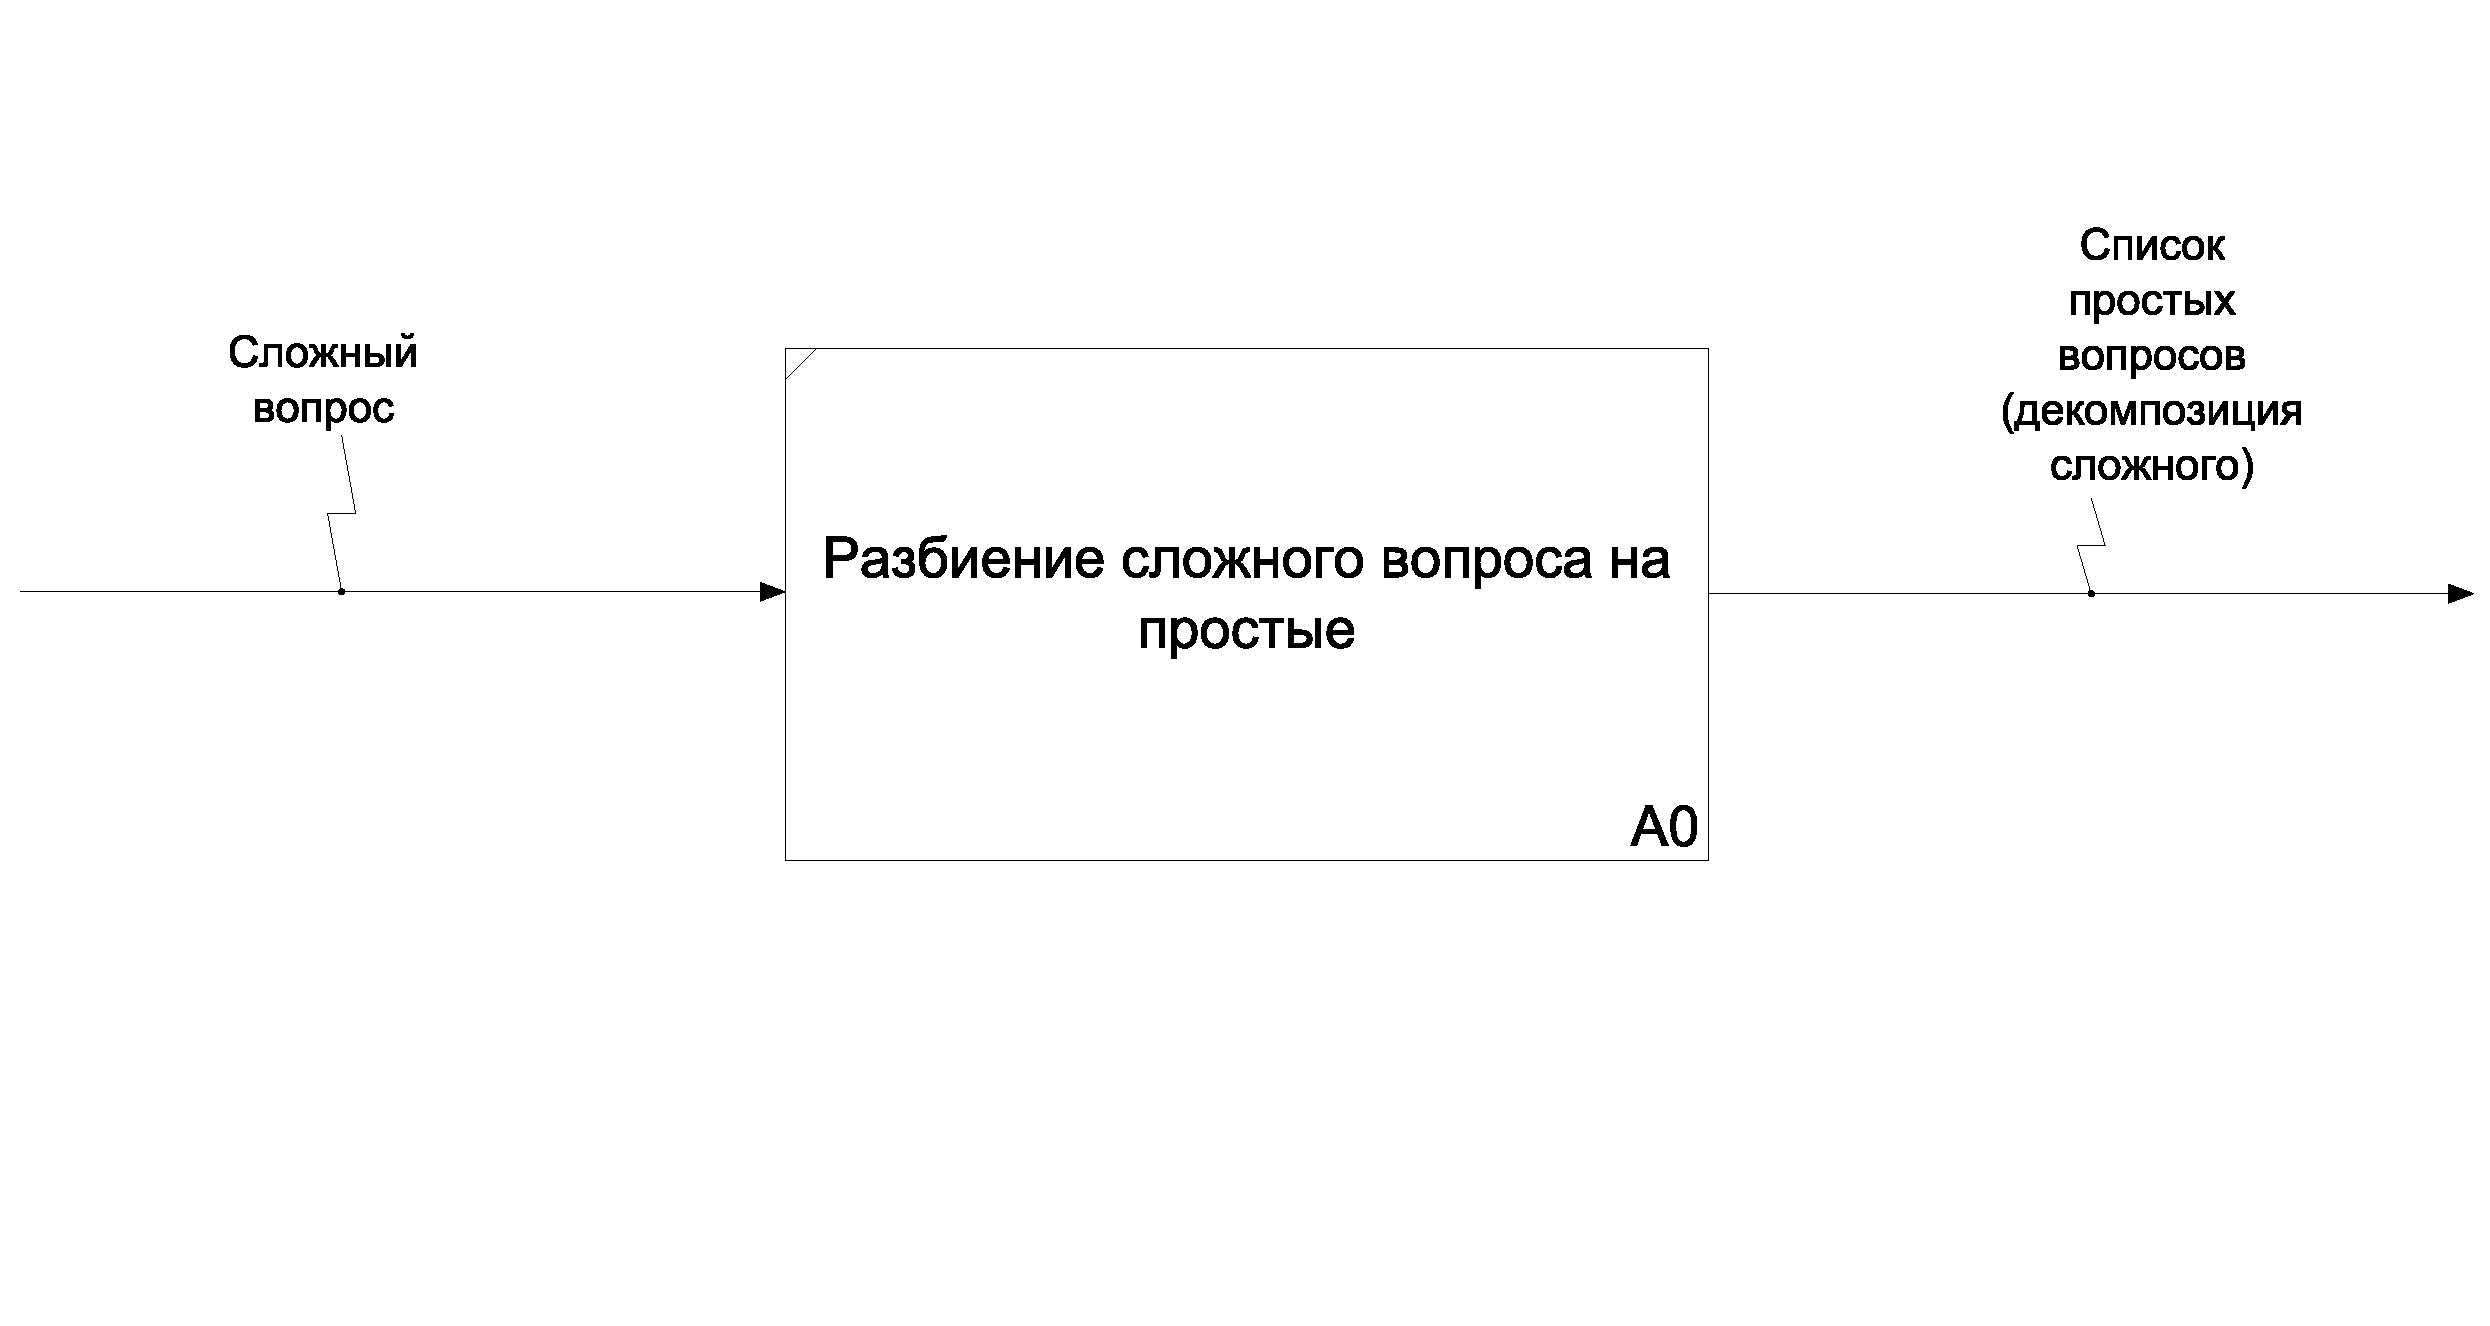
\includegraphics[width=0.8\textwidth]{images/analyth_idef0.pdf}
	\caption{Функциональная модель процесса разбиения сложных вопросов на простые}
	\label{fig:idef0}
\end{figure}

\section{Вывод}

В аналитическом разделе был проведен комплексный анализ задачи разбиения сложных вопросов на простые. Рассмотрены основные проблемы и требования к процессу декомпозиции, исследованы существующие подходы в трёх категориях: экспертная оценка, алгоритмические методы и методы на основе больших языковых моделей. Проанализировано более 30 существующих решений с точки зрения их применимости к решению поставленной задачи.

На основе проведенного анализа разработана функциональная модель процесса, в которой декомпозиция вопроса осуществляется с помощью языковой модели. Такой подход позволяет эффективно решать поставленную задачу, обеспечивая необходимую гибкость и качество результатов при минимальных требованиях к разработке дополнительных компонентов системы.